\documentclass[preprint]{aastex}
\begin{document}
\begin{figure}%[hbt!]
%\centering
\\
\mbox{
          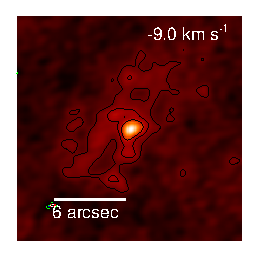
\includegraphics[]{test__34.ps}
          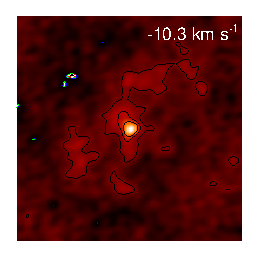
\includegraphics[]{test__35.ps}
          }
\\
\mbox{
          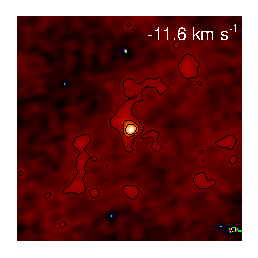
\includegraphics[]{test__36.ps}
          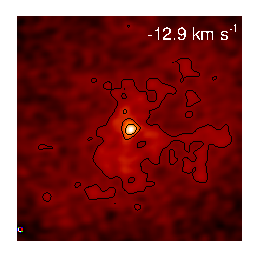
\includegraphics[]{test__37.ps}
          }
\\
\mbox{
          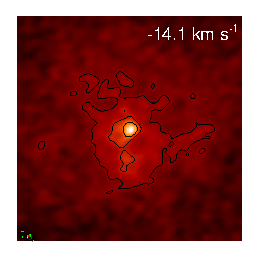
\includegraphics[]{test__38.ps}
          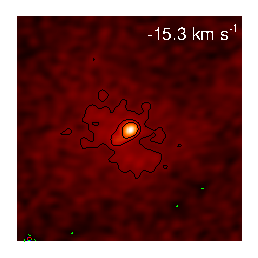
\includegraphics[]{test__39.ps}
          }
\\
\mbox{
          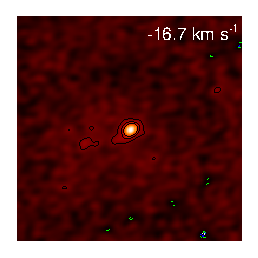
\includegraphics[]{test__40.ps}
          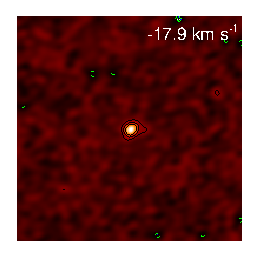
\includegraphics[]{test__41.ps}
          }
          \caption{Channel maps with no emission cut showing an expanded view of the star where the bright
emission is. More difficult to see the formation of S2 in this view.}
\end{figure}

\end{document}